\chapter{On Formal Grammars}

Chomsky defines a grammar as a ``device that enumerates the sentences of a language'' and proposes a set of restrictions that limit these grammars to different types of automata \cite{chomsky-hierarchy}, as seen in \ref{fig:chomsky-fig}

\begin{figure}[h]
    \centering
    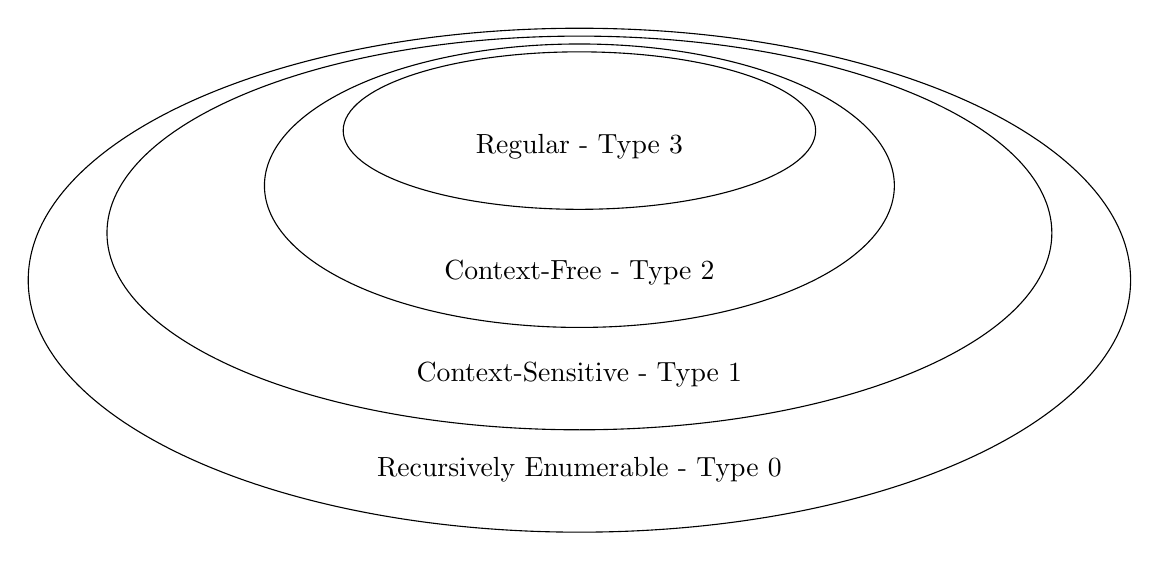
\begin{tikzpicture}
        % Draw ellipses for each language class
        \draw (0, -0.2) ellipse (7 and 3.2);
        \draw (0, 0.4) ellipse (6 and 2.5);
        \draw (0, 1) ellipse (4 and 1.8);
        \draw (0, 1.7) ellipse (3 and 1);
    
        % Add labels inside each ellipse
        \node at (0, -2.6) {Recursively Enumerable - Type 0};
        \node at (0, -1.4) {Context-Sensitive - Type 1};
        \node at (0, -0.1) {Context-Free - Type 2};
        \node at (0, 1.5) {Regular - Type 3};
    
    \end{tikzpicture}
    \caption{Chomsky Hierarchy}
    \label{fig:chomsky-fig}
\end{figure}

Regarding recognition, recursively enumerable grammars are recognized by Turing machines, Type 1 grammars are recognized by linearly bound non-deterministic Turing machines, Type 2 (or Context-Free Grammars) are recognized by a non-deterministic pushdown automaton and regular grammars are recognized by finite state machines.

Chomsky's hierarchy is defined in a way that the ``languages that can be generated by grammars meeting a given restriction constitute a proper subset of those that can be generated by grammars meeting the preceding restriction" \cite{chomsky-hierarchy}



\section{Context-Free Grammars}

\section{Dyck-$k$ Languages}